\documentclass{beamer}
\usepackage{etex}
\usepackage{booktabs}
\usepackage{xspace}

\usepackage{ifthen}
\usepackage[utf8]{inputenc}
\usepackage{lmodern}

\setbeamertemplate{navigation symbols}{}
\setbeamertemplate{headline}{}
\setbeamertemplate{footline}
{\hfill\insertframenumber{} /\inserttotalframenumber\hspace*{1ex}}

% Define my settings
\definecolor{mygreen}{cmyk}{0.82,0.11,1,0.25}
\setbeamercolor{structure}{fg=blue}
%packages indispensables 

%packages utiles
\usepackage{alltt} %program code
\usepackage{amssymb} %lettres mathématiques
\usepackage{amsmath}
\usepackage{amsthm}
\usepackage{bussproofs} %derivation
\usepackage{hyperref} %to write path.
\usepackage{color} % colouring text
\usepackage{tabularx} % table
\usepackage{graphicx}
\usepackage{enumerate}

\def\cakeml{\textsf{CakeML}\xspace}
\def\holfour{\textsf{HOL4}\xspace}
\def\isabellehol{\textsf{Isabelle/HOL}\xspace}
\def\hollight{\textsf{HOL Light}\xspace}
\def\coq{\textsf{Coq}\xspace}
\def\ocaml{\textsf{OCaml}\xspace}
\def\sml{\textsf{SML}\xspace}
\def\holyhammer{\textsf{HOL(y)Hammer}\xspace}
\def\vampire{\textsf{Vampire}\xspace}
\def\eprover{\textsf{E~prover}\xspace}
\def\zthree{\textsf{Z3}\xspace}
\def\metis{\textsf{Metis}\xspace}
\def\o{\scriptsize{$\emptyset$}}
\def\tactictoe{\textsf{TacticToe}\xspace}
% GRAPHICS
\usepackage{graphicx} % margin definition
\usepackage{pgfplots} % graphics
\usepackage{tikz} % graphics
% graphs
\usetikzlibrary{arrows,shapes,calc}
\usetikzlibrary{trees,positioning,fit}
\tikzstyle{arrow}=[draw,-to,thick]
\tikzstyle{bluearrow}=[draw,-to,thick,blue]
\tikzstyle{tcircle} = [circle, draw, fill=white]
\tikzstyle{bcircle} = [circle, draw, blue, fill=blue]
\tikzstyle{gcircle} = [circle, draw, mygreen, fill=mygreen]

\tikzstyle{block} =
  [rectangle, draw,
   minimum width=9em, text centered, rounded corners, minimum height=2.0em]
\tikzstyle{line}=[draw]
\tikzstyle{cloud} =
  [draw, text centered, ellipse, minimum height=2.0em, minimum width=9em]

\title{Learning to Prove with Tactics} 
\author{Thibault Gauthier, 
Cezary Kaliszyk, Josef Urban, Ramana~Kumar, Michael Norrish} 

\usepackage[final]{listings}
%\usepackage[scaled=.95]{couriers}
\lstdefinelanguage{SMLSmall}%
{columns=fixed,
  keywords={THEN,THENL,val,open,store_thm,fun,fn,let,in,end,true,
  while,do,if,then,else,break,return,;},%
  frame=none,
  sensitive=true,
  keywordstyle=\fontfamily{lmss}\scriptsize\selectfont,%
  basicstyle=\fontfamily{pcr}\small\selectfont,%
  stringstyle=\tt,
  morestring=[b]",
  literate=
   {=}{{\tt\raisebox{-.15mm}{=}}}1%
   {[}{{\tt\raisebox{-.15mm}{[}}}1%
   {]}{{\tt\raisebox{-.15mm}{]}}}1%
   {->}{{$\rightarrow$}}1%
   {wedge}{{$\wedge$}}1%
   {vee}{{$\vee$}}1%
   {==>}{{$\Rightarrow$}}1%
   {<==>}{{$\Leftrightarrow$}}1%
   {vee}{{$\vee$}}1%
   {<=}{{$\leq$}}1%
   {>=}{{$\geq$}}1%
   {'a}{{$\alpha$}}1%
   {'b}{{$\beta$}}1%
   {ldots}{$\ldots$}1%
   {emptyset}{$\emptyset$}1%
   {!}{$\forall$}1%
   {fff}{{DB.fetch}}1%
   {``}{\hspace{-.5mm}`\hspace{-1mm}`}1%
  }
\lstset{language=SMLSmall}
\begin{document}

\begin{frame}
\titlepage
\end{frame}

\begin{frame}{Problem}

Can we formally prove mathematical formulas automatically?

\end{frame}


\begin{frame}{Our solution}

\begin{center}
\begin{tikzpicture}[node distance = 1.5cm]
  \node [] (aa) {\textbf{Supervised learning}};
  \only<1> 
  {\node [cloud, below of=aa, node distance = 1cm] (a) {Formal 
  library};}
  \only<2> 
  {\node [cloud, below of=aa, node distance = 1cm, blue] (a) {Formal 
  library};}
  
  \node [block, below of=a] (b) {Proof recording};
  \node [cloud, below of=b] (c) {Knowledge base};
  \node [block, below of=c] (e) {Training};
  \node [block, below of=e] (d) {Predictors};

  \draw [-to,black,thick] (a) to (b);
  \draw [-to,black,thick] (b.south) to (c.north);
  \draw [-to,black,thick] (c) to [bend left]  (e);
  \draw [-to,black,thick] (e) to [bend left]  (c);
  \draw [-to,black,thick] (c.east) to [out=330,in=30] (d);

  \node [right of=aa, node distance=6.2cm] (0) {\textbf{Proving}};
  \node [cloud, below of=0, node distance = 1cm] (1) {Conjecture};
  \node [cloud, below of=1, node distance = 1.3cm] (2) {Search tree};
  \node [block, below of=2, node distance=1.1cm] (3) {Tactic policy};
  \node [above of=2, xshift=-16mm, node distance = 0.7cm] (00) {Proof
  search};
  \node [block, below of=3, node distance = 1.3cm] (4) {Tactic evaluation};
  \node [block, fit=(2) (3) (4)] (5) {};
  \node [block, below of=4, node distance = 1.3cm] (6) {Proof minimization};
  \node [cloud, below of=6, node distance = 1.3cm] (7) {Proof};
  \draw [-to,black,thick] (1) to (5);
  \draw [-to,black,thick] (5) to (6);
  \draw [-to,black,thick] (6) to (7);
  \draw [-to,black,thick] (d) to [out=0, in=180] (3);
  \draw [-to,black,thick] (d) to [out=0, in=180] (4);
\end{tikzpicture}
\end{center}
\end{frame}


\begin{frame}{Formal library: reasoning with inference rules}

 \begin{center}
 	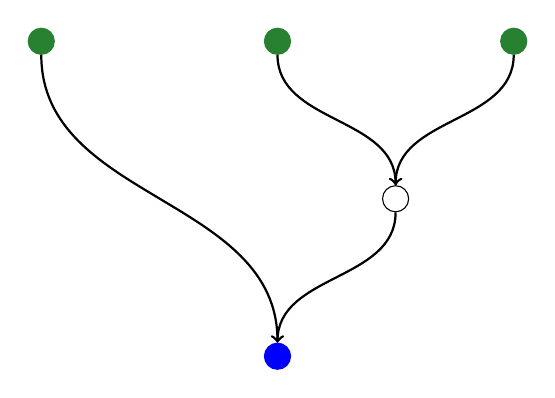
\begin{tikzpicture}[node distance=3cm]
 	\node [gcircle] (1) {};
 	\node [gcircle,right of=1] (2) {};
 	\node [gcircle,right of=2] (3) {};
    \node[right of=2,node distance=1.5cm] (m23) {};
    \uncover<2-3>{\node [tcircle, below of=m23,node distance=2cm] (4) {};
                  \draw[-to,thick] (3) to [out=270,in=90] (4);
                  \draw[-to,thick] (2) to [out=270,in=90] (4);
                 }
    \node [bcircle, below of=2,node distance=4cm] (5) {};
    \uncover<3-3>{
    	\draw[-to,thick] (1) to [out=270,in=90] (5);
    	\draw[-to,thick] (4) to [out=270,in=90] (5);
    }
 	
 	\end{tikzpicture}
 \end{center}


\begin{tikzpicture} \node[gcircle] {}; \end{tikzpicture} axiom \\

\begin{tikzpicture} \node[bcircle] {}; \end{tikzpicture} conjecture \\
$\rightarrow$ rule\\

\begin{tikzpicture} \node[tcircle] {}; \end{tikzpicture} lemma


\end{frame}

\begin{frame}{Formal library: reasoning with tactics}
 \begin{center}
 	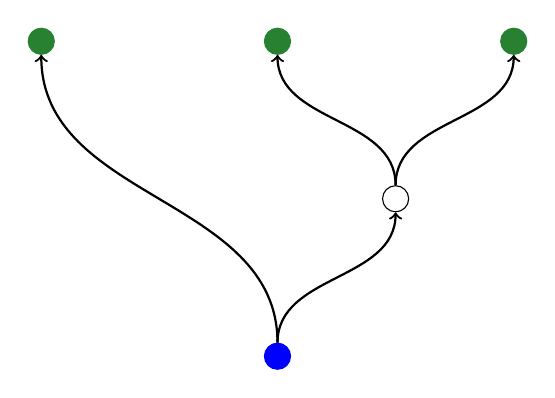
\begin{tikzpicture}[node distance=3cm]
 	\node [gcircle] (1) {};
 	\node [gcircle,right of=1] (2) {};
 	\node [gcircle,right of=2] (3) {};
 	\node[right of=2,node distance=1.5cm] (m23) {};
 	\uncover<2-3>{\node [tcircle, below of=m23,node distance=2cm] (4) {};}
 	\uncover<3-3>{
      \draw[-to,thick] (4) to [in=270,out=90] (3);
 	  \draw[-to,thick] (4) to [in=270,out=90] (2);
 	}
 	\node [bcircle, below of=2,node distance=4cm] (5) {};
 	\uncover<2-3>{
 		\draw[-to,thick] (5) to [in=270,out=90] (1);
 		\draw[-to,thick] (5) to [in=270,out=90] (4);
 	}
 	\end{tikzpicture}
  \end{center}

\vspace{5mm}


\begin{tikzpicture} \node[gcircle] {}; \end{tikzpicture} axiom\\

\begin{tikzpicture} \node[bcircle] {}; \end{tikzpicture} conjecture\\
$\rightarrow$ tactic\\

\begin{tikzpicture} \node[tcircle] {}; \end{tikzpicture} goal\\

\end{frame}

\begin{frame}{Formal library: tactics}

\texttt{REWRITE\_TAC}

\vspace{5mm}

\texttt{INDUCT\_TAC}

\vspace{5mm}

\texttt{METIS\_TAC}

\end{frame}

\begin{frame}{Formal library: composing tactics}
\centering
\texttt{THENL} tactical composes the effect of tactics.\\
\vspace{5mm}

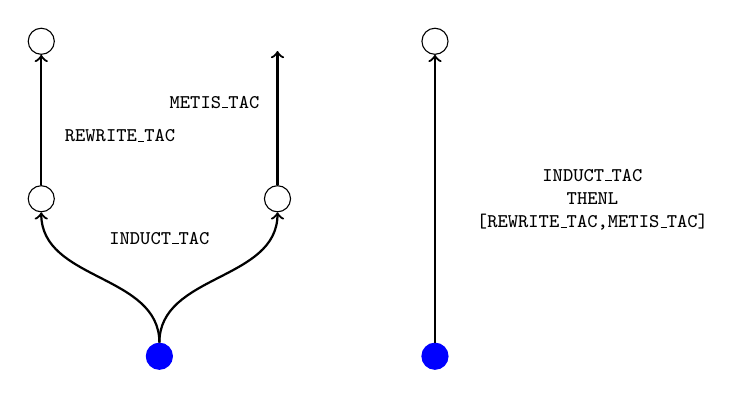
\begin{tikzpicture}[node distance=3cm]
\uncover<3->{\node [tcircle] (1) {};}
\uncover<3->{\node [right of=1] (2) {};}

\node [right of=1,node distance=1.5cm] (m12) {};
\uncover<5->{\node [tcircle,right of=2,node distance=2cm] (l1) {};}

\uncover<2->{
\node [tcircle, below of=1,node distance=2cm] (b1) {};
\node [tcircle, below of=2,node distance=2cm] (b2) {};
}
\uncover<3->{
\draw[-to,thick] (b1) to node [xshift=10mm,yshift=-2mm] {\scriptsize 
\texttt{REWRITE\_TAC}} (1);
\draw[-to,thick] (b2) to node [xshift=-8mm,yshift=2mm] {\scriptsize 
\texttt{METIS\_TAC}} (2);
}
\node [bcircle, below of=m12,node distance=4cm] (cj1) {};
\uncover<4->{\node [bcircle, below of=l1,node distance=4cm] (cj2) {};}
\uncover<5->{
\draw[-to,thick] (cj2) to (l1);
\node [below of=l1,node distance=2cm,yshift=3mm,xshift=20mm] () 
{\scriptsize \texttt{INDUCT\_TAC}};
\node [below of=l1,node distance=2cm,yshift=0mm,xshift=20mm] () 
{\scriptsize \texttt{THENL}};
\node [below of=l1,node distance=2cm,yshift=-3mm,xshift=20mm] () 
{\scriptsize \texttt{[REWRITE\_TAC,METIS\_TAC]}};
}

\uncover<2->{
\node [below of=m12,node distance=2.5cm] () {\scriptsize \texttt{INDUCT\_TAC}};
\draw[-to,thick] (cj1) to [out=90,in=270] (b1);
\draw[-to,thick] (cj1) to [out=90,in=270] (b2);
}
\end{tikzpicture}
\end{frame}

\begin{frame}{}
\centering \Large Demo
\end{frame}

\begin{frame}{Plan}
\begin{center}
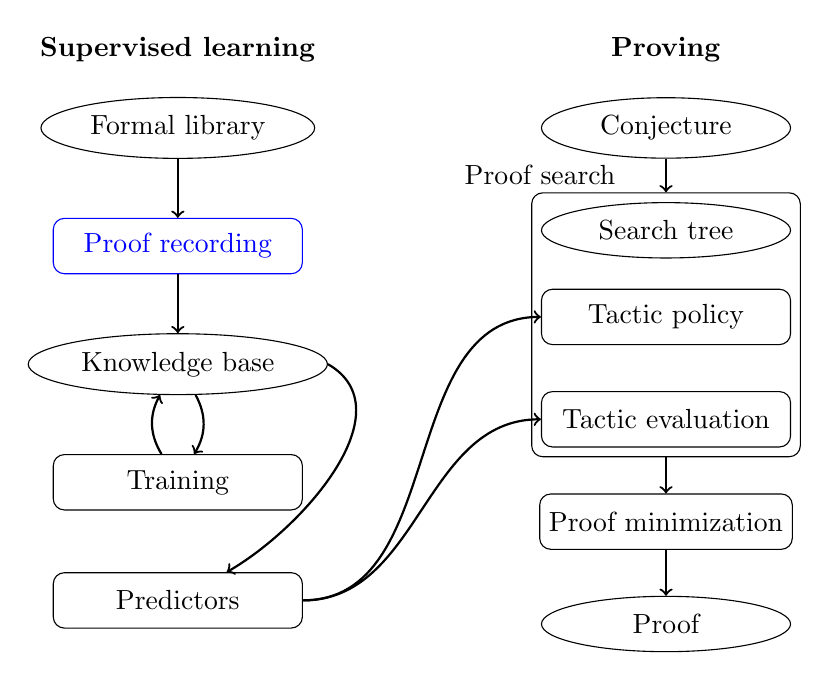
\begin{tikzpicture}[node distance = 1.5cm]
  \node [] (aa) {\textbf{Supervised learning}};
  \node [cloud, below of=aa, node distance = 1cm] (a) {Formal library};
  \node [block, blue, below of=a] (b) {Proof recording};
  \node [cloud, below of=b] (c) {Knowledge base};
  \node [block, below of=c] (e) {Training};
  \node [block, below of=e] (d) {Predictors};

  \draw [-to,black,thick] (a) to (b);
  \draw [-to,black,thick] (b.south) to (c.north);
  \draw [-to,black,thick] (c) to [bend left]  (e);
  \draw [-to,black,thick] (e) to [bend left]  (c);
  \draw [-to,black,thick] (c.east) to [out=330,in=30] (d);

  \node [right of=aa, node distance=6.2cm] (0) {\textbf{Proving}};
  \node [cloud, below of=0, node distance = 1cm] (1) {Conjecture};
  \node [cloud, below of=1, node distance = 1.3cm] (2) {Search tree};
  \node [block, below of=2, node distance=1.1cm] (3) {Tactic policy};
  \node [above of=2, xshift=-16mm, node distance = 0.7cm] (00) {Proof
  search};
  \node [block, below of=3, node distance = 1.3cm] (4) {Tactic 
  evaluation};
  \node [block, fit=(2) (3) (4)] (5) {};
  \node [block, below of=4, node distance = 1.3cm] (6) {Proof minimization};
  \node [cloud, below of=6, node distance = 1.3cm] (7) {Proof};
  \draw [-to,black,thick] (1) to (5);
  \draw [-to,black,thick] (5) to (6);
  \draw [-to,black,thick] (6) to (7);
  \draw [-to,black,thick] (d) to [out=0, in=180] (3);
  \draw [-to,black,thick] (d) to [out=0, in=180] (4);
\end{tikzpicture}
\end{center}
\end{frame}


\begin{frame}[fragile]{Recording}
Original proof:
\begin{lstlisting}[language=SMLSmall]
INDUCT_TAC THENL [REWRITE_TAC, METIS_TAC]
\end{lstlisting}

Modified proof:
\begin{lstlisting}[language=SMLSmall]
(R numLib.INDUCT_TAC) THENL 
  [R boolLib.REWRITE_TAC, R metisLib.METIS_TAC]
\end{lstlisting}

Database of tactics:
\begin{lstlisting}[language=SMLSmall]
R (f n) (f (SUC n)) ==> transitive R: INDUCT_TAC
n * m <= n * p ==> (n = 0) vee m <= p   : REWRITE_TAC
INJ f U(:num) s ==> INFINITE s      : METIS_TAC
ldots
\end{lstlisting}
\end{frame}

\begin{frame}{Plan}
\begin{center}
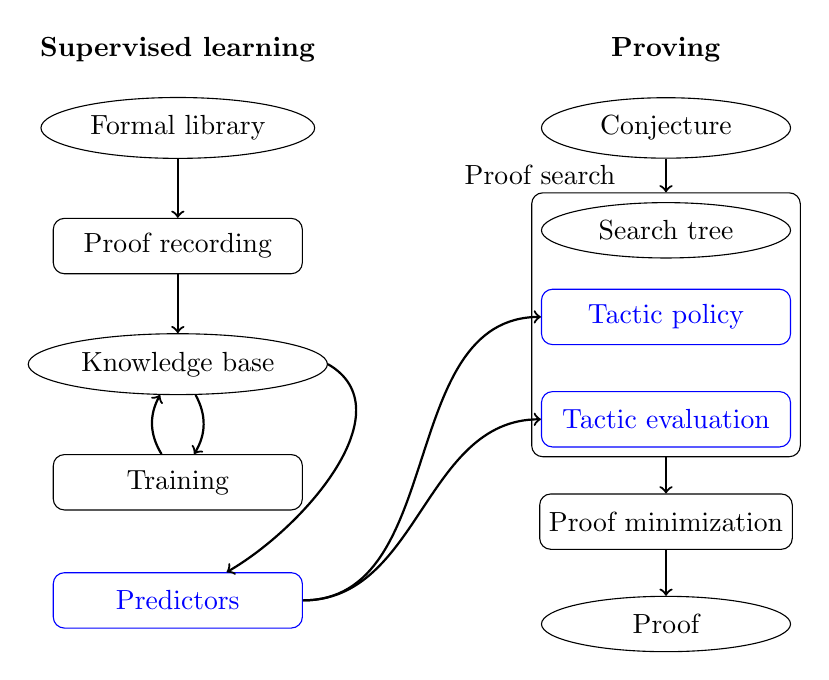
\begin{tikzpicture}[node distance = 1.5cm]
  \node [] (aa) {\textbf{Supervised learning}};
  \node [cloud, below of=aa, node distance = 1cm] (a) {Formal library};
  \node [block, below of=a] (b) {Proof recording};
  \node [cloud, below of=b] (c) {Knowledge base};
  \node [block, below of=c] (e) {Training};
  \node [block, blue, below of=e] (d) {Predictors};

  \draw [-to,black,thick] (a) to (b);
  \draw [-to,black,thick] (b.south) to (c.north);
  \draw [-to,black,thick] (c) to [bend left]  (e);
  \draw [-to,black,thick] (e) to [bend left]  (c);
  \draw [-to,black,thick] (c.east) to [out=330,in=30] (d);

  \node [right of=aa, node distance=6.2cm] (0) {\textbf{Proving}};
  \node [cloud, below of=0, node distance = 1cm] (1) {Conjecture};
  \node [cloud, below of=1, node distance = 1.3cm] (2) {Search tree};
  \node [block, below of=2, blue, node distance=1.1cm] (3) {Tactic policy};
  \node [above of=2, xshift=-16mm, node distance = 0.7cm] (00) {Proof
  search};
  \node [block, below of=3, blue, node distance = 1.3cm] (4) {Tactic 
  evaluation};
  \node [block, fit=(2) (3) (4)] (5) {};
  \node [block, below of=4, node distance = 1.3cm] (6) {Proof minimization};
  \node [cloud, below of=6, node distance = 1.3cm] (7) {Proof};
  \draw [-to,black,thick] (1) to (5);
  \draw [-to,black,thick] (5) to (6);
  \draw [-to,black,thick] (6) to (7);
  \draw [-to,black,thick] (d) to [out=0, in=180] (3);
  \draw [-to,black,thick] (d) to [out=0, in=180] (4);
\end{tikzpicture}
\end{center}
\end{frame}


\begin{frame}{Prediction algorithm}

Algorithm:\\ \ \  
  Nearest neighbor weighted by TF-IDF heuristics

\vspace{5mm}

Effect:\\ \ \
  Order goals from the database according to\\
  their distance to a target goal.

\vspace{5mm}

Remark:\\ \ \ 
  This is algorithm performs premise selection.\\ \ \
  How do we adapt it to predict tactics?

\end{frame}

\begin{frame}[fragile]{Policy: choosing a tactic}

Database of tactics is a map from goals to tactics.
\begin{lstlisting}[language=SMLSmall]
R (f n) (f (SUC n)) ==> transitive R: INDUCT_TAC
n * m <= n * p ==> (n = 0) vee m <= p   : REWRITE_TAC
INJ f U(:num) s ==> INFINITE s      : METIS_TAC
ldots
\end{lstlisting}
An order on goals induces an order on tactics.


Goal appearing during proof search:
\begin{lstlisting}[language=SMLSmall]
LENGTH (MAP f l) = LENGTH l
\end{lstlisting}

Policy for the new goal:
\begin{lstlisting}[language=SMLSmall]
Rank Tactic      Policy
1    REWRITE_TAC 0.5 
2    METIS_TAC   0.25
ldots 
4    INDUCT_TAC  0.0625
ldots
\end{lstlisting}
\end{frame}

\begin{frame}{Value function: provability of a list of goals}
Database of lists of goals:\\
\begin{itemize}
\item Positive examples: appears in human proofs.
\item Negative examples: produced during \tactictoe search but do not appear in 
the final proof.
\end{itemize}

Value function:\\
\ \ Percentage of positives in the 10 closest lists of goals of a target list 
of goals. 

\vspace{5mm}

Future work:\\
\ \ Estimate the number of steps needed to prove a list of goals.

\end{frame}

\begin{frame}{Plan}
\begin{center}
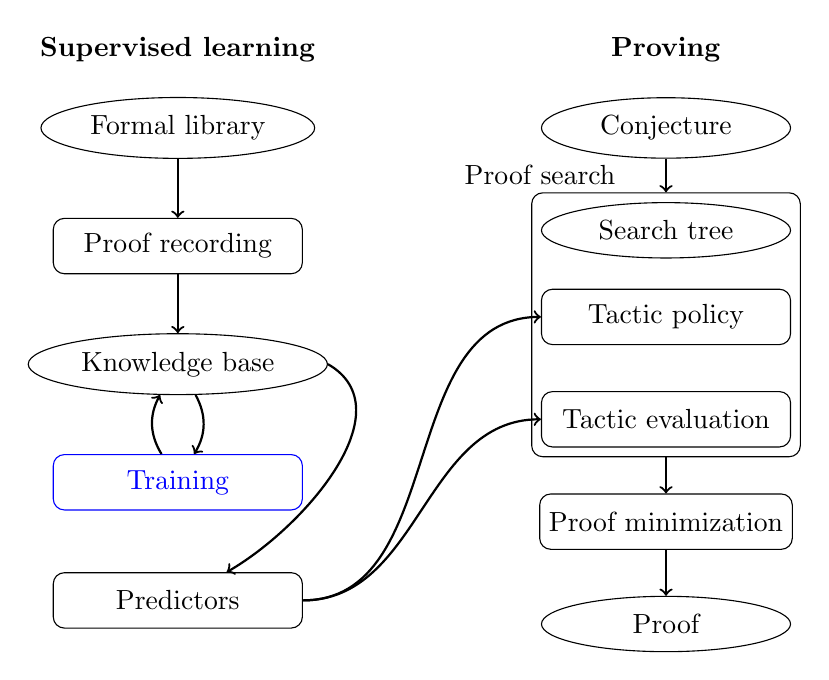
\begin{tikzpicture}[node distance = 1.5cm]
  \node [] (aa) {\textbf{Supervised learning}};
  \node [cloud, below of=aa, node distance = 1cm] (a) {Formal library};
  \node [block, below of=a] (b) {Proof recording};
  \node [cloud, below of=b] (c) {Knowledge base};
  \node [block, below of=c, blue] (e) {Training};
  \node [block, below of=e] (d) {Predictors};

  \draw [-to,black,thick] (a) to (b);
  \draw [-to,black,thick] (b.south) to (c.north);
  \draw [-to,black,thick] (c) to [bend left]  (e);
  \draw [-to,black,thick] (e) to [bend left]  (c);
  \draw [-to,black,thick] (c.east) to [out=330,in=30] (d);

  \node [right of=aa, node distance=6.2cm] (0) {\textbf{Proving}};
  \node [cloud, below of=0, node distance = 1cm] (1) {Conjecture};
  \node [cloud, below of=1, node distance = 1.3cm] (2) {Search tree};
  \node [block, below of=2, node distance=1.1cm] (3) {Tactic policy};
  \node [above of=2, xshift=-16mm, node distance = 0.7cm] (00) {Proof
  search};
  \node [block, below of=3, node distance = 1.3cm] (4) {Tactic 
  evaluation};
  \node [block, fit=(2) (3) (4)] (5) {};
  \node [block, below of=4, node distance = 1.3cm] (6) {Proof minimization};
  \node [cloud, below of=6, node distance = 1.3cm] (7) {Proof};
  \draw [-to,black,thick] (1) to (5);
  \draw [-to,black,thick] (5) to (6);
  \draw [-to,black,thick] (6) to (7);
  \draw [-to,black,thick] (d) to [out=0, in=180] (3);
  \draw [-to,black,thick] (d) to [out=0, in=180] (4);
\end{tikzpicture}
\end{center}
\end{frame}




\begin{frame}{Training}

Improve recorded data to create better predictions during search.

\end{frame}


\begin{frame}[fragile]{Training: orthogonalization}

Issue: Many tactics are doing the same job on a goal $g$.

\vspace{5mm}

Solution: Competition for $g$ where the most popular tactic wins.
\end{frame}


\begin{frame}[fragile]{Training: orthogonalization}

Recorded goal-tactic pair:
\begin{lstlisting}[language=SMLSmall]
LENGTH (MAP f l) = LENGTH l: INDUCT_TAC
\end{lstlisting}

Competition:
\begin{lstlisting}[language=SMLSmall]
            Progress  Coverage 
INDUCT_TAC  Yes       136
REWRITE_TAC No        2567
METIS_TAC   Yes       694
\end{lstlisting}

Added to the database:
\begin{lstlisting}[language=SMLSmall]
LENGTH (MAP f l) = LENGTH l: METIS_TAC
\end{lstlisting}
\end{frame}

\begin{frame}{Training: abstraction}
Issue: Some theorems are never used inside tactics.

\vspace{5mm}

Solution: Abstract all lists of theorems in a tactic\\ \ \ 
and instantiate them depending on the target goal.
\end{frame}

\begin{frame}[fragile]{Training: abstraction}

Abstraction algorithm:
\begin{lstlisting}[language=SMLSmall]
Original     : REWRITE_TAC [T1,T2]
Abstraction  : REWRITE_TAC X
Instantiation: REWRITE_TAC [T67, T1, T43, ldots]
\end{lstlisting}

\vspace{5mm}

Question: Dow we keep the original or the abstraction ?\\

\vspace{5mm}

Answer: Let them compete during orthogonalization.\\

\end{frame}

\begin{frame}{Training: preselection}

Issue: Predictions are too slow during proof search.

\vspace{5mm}

Solution: Preselect 1000 suitable tactics using dependencies.

\vspace{5mm}

Dependency: Appear in the same proof.

\end{frame}

\begin{frame}{Plan}
\begin{center}
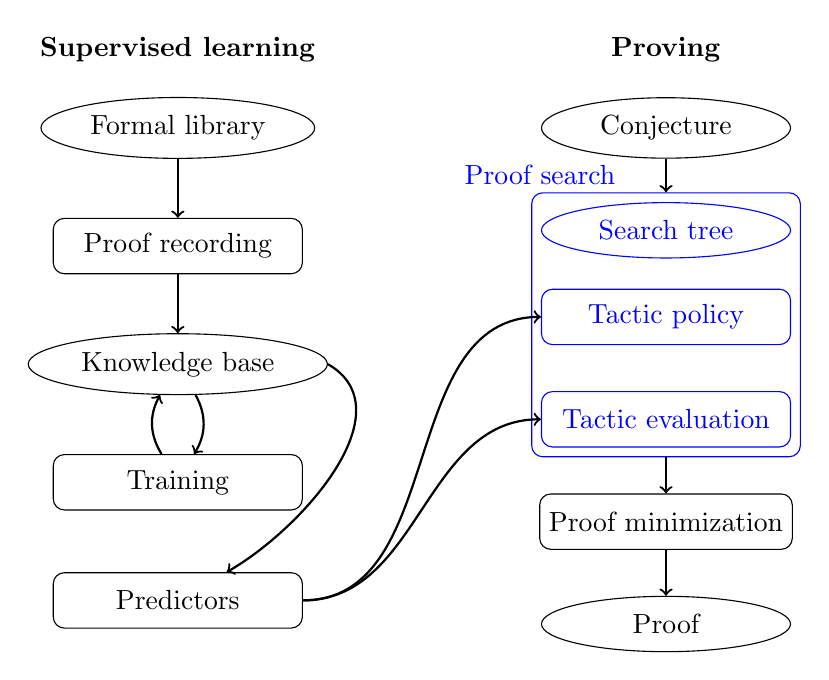
\begin{tikzpicture}[node distance = 1.5cm]
  \node [] (aa) {\textbf{Supervised learning}};
  \node [cloud, below of=aa, node distance = 1cm] (a) {Formal library};
  \node [block, below of=a] (b) {Proof recording};
  \node [cloud, below of=b] (c) {Knowledge base};
  \node [block, below of=c] (e) {Training};
  \node [block, below of=e] (d) {Predictors};

  \draw [-to,black,thick] (a) to (b);
  \draw [-to,black,thick] (b.south) to (c.north);
  \draw [-to,black,thick] (c) to [bend left]  (e);
  \draw [-to,black,thick] (e) to [bend left]  (c);
  \draw [-to,black,thick] (c.east) to [out=330,in=30] (d);

  \node [right of=aa, node distance=6.2cm] (0) {\textbf{Proving}};
  \node [cloud, below of=0, node distance = 1cm] (1) {Conjecture};
  \node [cloud, below of=1, blue, node distance = 1.3cm] (2) {Search tree};
  \node [block, below of=2, blue, node distance=1.1cm] (3) {Tactic policy};
  \node [above of=2, xshift=-16mm, blue, node distance = 0.7cm] (00) {Proof
  search};
  \node [block, below of=3, blue, node distance = 1.3cm] (4) {Tactic 
  evaluation};
  \node [block, blue, fit=(2) (3) (4)] (5) {};
  \node [block, below of=4, node distance = 1.3cm] (6) {Proof minimization};
  \node [cloud, below of=6, node distance = 1.3cm] (7) {Proof};
  \draw [-to,black,thick] (1) to (5);
  \draw [-to,black,thick] (5) to (6);
  \draw [-to,black,thick] (6) to (7);
  \draw [-to,black,thick] (d) to [out=0, in=180] (3);
  \draw [-to,black,thick] (d) to [out=0, in=180] (4);
\end{tikzpicture}
\end{center}
\end{frame}

\begin{frame}{Proof search: search tree}
\centering
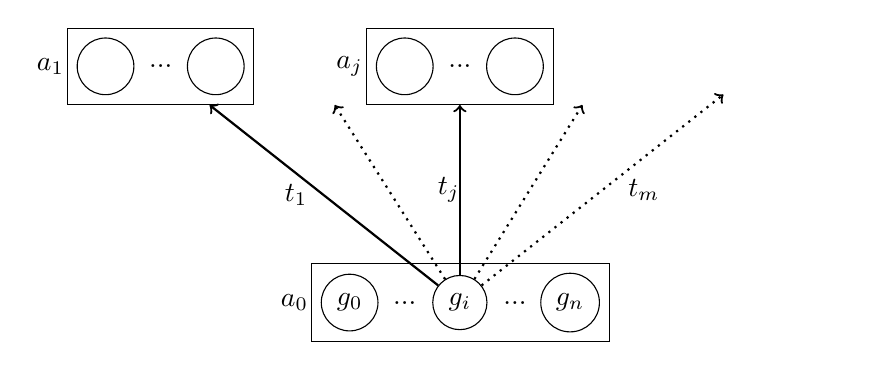
\begin{tikzpicture}[node distance=0.7cm]
\node [tcircle] (0) {$g_i$};
\node [right of=0] (0r) {...};
\node [tcircle,right of=0r] (0rr) {$g_n$};
\node [left of=0] (0l) {...};
\node [tcircle,left of=0l] (0ll) {$g_0$};
\node [draw,fit=(0rr) (0ll)] (0b) {};
\node [left of=0ll] {$a_0$};
\node [above of=0,node distance=3cm] (2) {...};
\node [left of=2, tcircle] (2l) {$\phantom{g_3}$};
\node [tcircle,right of=2] (2r) {$\phantom{g_3}$};
\node [draw, fit=(2l) (2r)] (2b) {};
\node [left of=2l] {$a_j$};

\node [tcircle, left of=2l, node distance=2.4cm] (1r) {$\phantom{g_3}$};
\node [left of=1r] (1) {...};
\node [tcircle, left of=1] (1l) {$\phantom{g_3}$};
\node [draw, fit=(1l) (1r)] (1b) {};
\node [left of=1l] {$a_1$};

\node [right of=2r,node distance=2.4cm] (3l) {$\phantom{g_3}$};
\node [right of=3l] (3) {\phantom{...}};
\node [right of=3] (3r) {$\phantom{g_3}$};
\node [fit=(3l) (3r)] (3b) {};

\node [fit=(1r) (2l)] (1m) {};
\node [fit=(2l) (3r)] (2m) {};

\draw[-to,thick] (0) to node[xshift=-10](t1){$t_1$} (1b);
\draw[-to,thick] (0) to node[xshift=-4](t2){$t_j$} (2b);
\draw[-to,dotted,thick] (0) to (1m);
\draw[-to,dotted,thick] (0) to (2m);
\draw[-to,dotted,thick] (0) to node[xshift=15](t2){$t_m$} (3b);
\end{tikzpicture}
\end{frame}


\begin{frame}{Proof search: advanced tree search}
\begin{center}
\begin{tikzpicture}[node distance=3cm]

\node [tcircle] (0) {\only<1>{}\only<2>{0.7}\only<3>{0.5}\only<4->{0.6}};
\node [tcircle, above of=0] (1) {\only<4->{0.8}};
\node [tcircle, left of=1] (2) {\only<2>{0.7}\only<3->{0.5}};
\node [tcircle, right of=1] (3) {};

\draw[-to,thick] (0) to node[xshift=15]{0.25} (1);
\draw[-to,thick] (0) to node[xshift=15]{0.5} (2);
\draw[-to,thick] (0) to node[xshift=20]{0.125} (3);

\uncover<2->{
\node [tcircle, above of=2] (4) {};
\node [tcircle, left of=4] (5) {\only<3->{0.3}};
\node [tcircle, right of=4] (6) {};

\draw[-to,thick] (2) to node[xshift=15]{0.25} (4);
\draw[-to,thick] (2) to node[xshift=15]{0.5} (5);
\draw[-to,thick] (2) to node[xshift=20]{0.125} (6);
}
\end{tikzpicture}
\end{center}
\end{frame}


\begin{frame}{Re-proving: results}
Evaluation is "fair". (not totally if you ask Freek)\\
Only previous proofs are available for training.

\begin{center}
\begin{tabular}{lcc}
\toprule
  & 7164 \holfour theorems (60s) & 3329 \cakeml theorems (15s)\\
\midrule
   \eprover   & 2472 (34.5\%) & \phantom{0000 } 20.0\%?\\
   \tactictoe & 4760 (66.4\%) & 1161 (34.9\%)\\
\midrule
   Total  & 4946 (69.0\%) & \\
\bottomrule
\end{tabular}
\end{center}
\end{frame}

\begin{frame}{Re-proving: number of proofs found in less that x seconds}
\pgfplotscreateplotcyclelist{my black}{
solid, mark repeat=100, mark phase=0, black!100\\
dashed, mark repeat=100, mark phase=0, black!100\\}

\centering
\begin{tikzpicture}[scale=1]
\begin{axis}[
  legend style={anchor=south east, at={(0.9,0.1)}},
  width=\textwidth,
  height=0.7*\textwidth,xmin=0, xmax=60,
  ymin=0, ymax=4800,
  xtick={},
  ytick={},
  cycle list name=my black]
\addplot table[x=time, y=solved] {data/tactictoe_time};
\addplot table[x=time, y=solved] {data/eprover_time};
\legend{\tactictoe,\eprover}
\end{axis}
\end{tikzpicture}
\end{frame}

\begin{frame}{Re-proving: number of human proofs of size x}
\pgfplotscreateplotcyclelist{my black}{
solid, mark repeat=100, mark phase=0, red!100\\
solid, mark repeat=100, mark phase=0, blue!100\\}

add cakeml
\centering
\begin{tikzpicture}[scale=1]
\begin{axis}[
  legend style={anchor=north east, at={(0.9,0.9)}},
  width=\textwidth,
  height=0.7*\textwidth,
  ymin=0, ymax=2000,
  xmin=0, xmax=20,
  xtick={},
  ytick={},
  cycle list name=my black]
\addplot table[x=length, y=proofs] {data/tactictoe_proof_length};
\legend{\holfour}
\end{axis}
\end{tikzpicture}
\end{frame}

\begin{frame}{Re-proving: percentage of proof of size x solved}
\pgfplotscreateplotcyclelist{my black}{
solid, mark repeat=100, mark phase=0, black!100\\
dashed, mark repeat=100, mark phase=0, black!100\\}

\centering
\begin{tikzpicture}[scale=1]
\begin{axis}[
  legend style={anchor=north east, at={(0.9,0.9)}},
  width=\textwidth,
  height=0.7*\textwidth,xmin=0, xmax=20,
  ymin=0, ymax=100,
  xtick={},
  ytick={},
  cycle list name=my black]
\addplot table[x=oplen, y=solved] {data/tactictoe_by_oplen};
\addplot table[x=oplen, y=solved] {data/eprover_by_oplen};
\legend{\tactictoe,\eprover}
\end{axis}
\end{tikzpicture}
\end{frame}


\begin{frame}{Plan}
\begin{center}
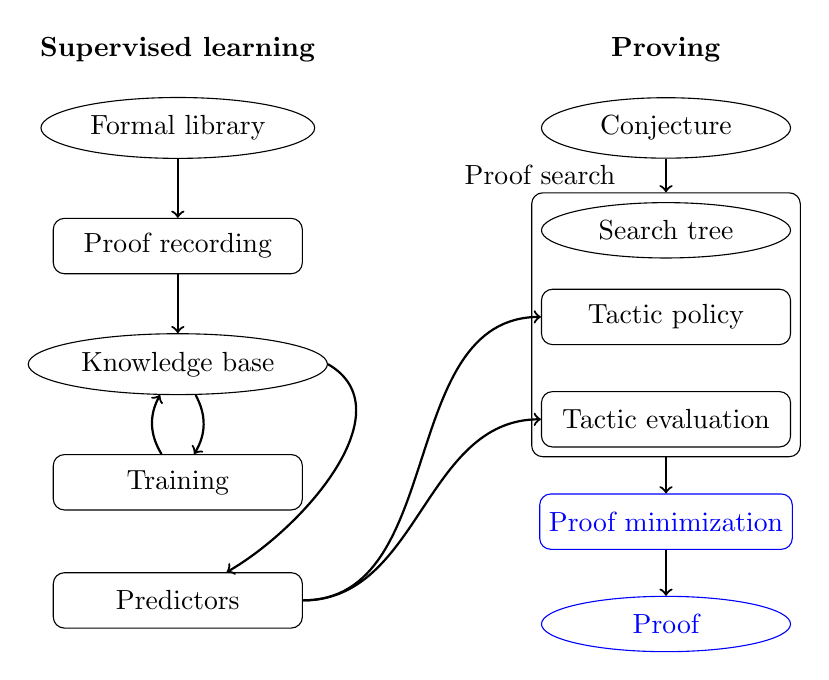
\begin{tikzpicture}[node distance = 1.5cm]
  \node [] (aa) {\textbf{Supervised learning}};
  \node [cloud, below of=aa, node distance = 1cm] (a) {Formal library};
  \node [block, below of=a] (b) {Proof recording};
  \node [cloud, below of=b] (c) {Knowledge base};
  \node [block, below of=c] (e) {Training};
  \node [block, below of=e] (d) {Predictors};

  \draw [-to,black,thick] (a) to (b);
  \draw [-to,black,thick] (b.south) to (c.north);
  \draw [-to,black,thick] (c) to [bend left]  (e);
  \draw [-to,black,thick] (e) to [bend left]  (c);
  \draw [-to,black,thick] (c.east) to [out=330,in=30] (d);

  \node [right of=aa, node distance=6.2cm] (0) {\textbf{Proving}};
  \node [cloud, below of=0, node distance = 1cm] (1) {Conjecture};
  \node [cloud, below of=1, node distance = 1.3cm] (2) {Search tree};
  \node [block, below of=2, node distance=1.1cm] (3) {Tactic policy};
  \node [above of=2, xshift=-16mm, node distance = 0.7cm] (00) {Proof
  search};
  \node [block, below of=3, node distance = 1.3cm] (4) {Tactic 
  evaluation};
  \node [block, fit=(2) (3) (4)] (5) {};
  \node [block, below of=4, blue, node distance = 1.3cm] (6) {Proof 
  minimization};
  \node [cloud, below of=6, blue, node distance = 1.3cm] (7) {Proof};
  \draw [-to,black,thick] (1) to (5);
  \draw [-to,black,thick] (5) to (6);
  \draw [-to,black,thick] (6) to (7);
  \draw [-to,black,thick] (d) to [out=0, in=180] (3);
  \draw [-to,black,thick] (d) to [out=0, in=180] (4);
\end{tikzpicture}
\end{center}
\end{frame}

\begin{frame}[fragile]{Minimization and embellishment}

Raw proof:
\begin{lstlisting}[language=SMLSmall]
boolLib.REWRITE_TAC [DB.fetch "list" "EVERY_CONJ",... ] 
  THEN
BasicProvers.Induct_on [HolKernel.QUOTE "l"] 
  THENL
  [BasicProvers.SRW_TAC [] [],
   simpLib.ASM_SIMP_TAC (BasicProvers.srw_ss ()) 
   [boolLib.DISJ_IMP_THM, DB.fetch "list" "MAP", 
    DB.fetch "list" "CONS_11", boolLib.FORALL_AND_THM]]
\end{lstlisting}

\vspace{5mm}
Processed proof:
\begin{lstlisting}[language=SMLSmall]
Induct_on `l` THENL
  [SRW_TAC [] [], 
   ASM_SIMP_TAC (srw_ss ()) 
   [DISJ_IMP_THM, FORALL_AND_THM]]
\end{lstlisting}

\end{frame}

\begin{frame}{Conclusion}
Summary: TacticToe learns from human proofs to solve new goals.

\vspace{5mm}

Advantages over ATPs (\eprover) for ITP (\holfour) users:
\begin{itemize}
\item Includes domain specific automation found in the ITP.
\item Generated proofs are human-level proofs.\\
\item No reconstruction needed.\\
\end{itemize}


\end{frame}

\begin{frame}{Future work}
Enlarge the action space:\\ \ \
  parameter synthesis, sequence of tactics, forward proofs.

\vspace{5mm}

Train tactics by evaluating input/output pairs.

\vspace{5mm}

Conjecture intermediate lemmas.
\vspace{5mm}
\end{frame}
 
\end{document}
